\documentclass[12pt,a4paper,twoside]{report}
\usepackage[margin=1in]{geometry}

\usepackage{fancyhdr, lastpage}
\pagestyle{fancy}
\fancyfoot{}

\usepackage{xargs}
\usepackage[pdftex,dvipsnames]{xcolor}
\usepackage{setspace}
\doublespacing

\usepackage[utf8]{inputenc}
\usepackage[T1]{fontenc}
\usepackage{textcomp}
\usepackage{amsmath,amssymb,mathtools}


% figure support
\usepackage{import}
\usepackage{xifthen}
\pdfminorversion=7
\usepackage{pdfpages}
\usepackage{transparent}
%\newcommand{\incfig}[1]{%
%	\def\svgwidth{\columnwidth}
%	\import{./figures/}{#1.pdf_tex}
%}

\newcommand{\incfig}[2][1]{%
    \def\svgwidth{#1\columnwidth}
    \import{./figures/}{#2.pdf_tex}
}
\usepackage{float}

%Options: Sonny, Lenny, Glenn, Conny, Rejne, Bjarne, Bjornstrup
%\usepackage[Glenn]{fncychap}

%%%%%%%%%%%%%%%%%%%%%%%%%%%%%%
%%%%%%%%%%%%%%%%%%%%%%%%%%%%%%
\usepackage[framemethod=TikZ]{mdframed}

%%%%%%%%%%%%%%%%%%%%%%%%%%%%%%
%Theorem
\newcounter{theo}[section] \setcounter{theo}{0}
\renewcommand{\thetheo}{\arabic{section}.\arabic{theo}}
\newenvironment{theo}[2][]{%
\refstepcounter{theo}%
\ifstrempty{#1}%
{\mdfsetup{%
frametitle={%
\tikz[baseline=(current bounding box.east),outer sep=0pt]
\node[anchor=east,rectangle,fill=blue!20]
{\strut Theorem~\thetheo};}}
}%
{\mdfsetup{%
frametitle={%
\tikz[baseline=(current bounding box.east),outer sep=0pt]
\node[anchor=east,rectangle,fill=blue!20]
{\strut Theorem~\thetheo:~#1};}}%
}%
\mdfsetup{innertopmargin=10pt,linecolor=blue!20,%
linewidth=2pt,topline=true,%
frametitleaboveskip=\dimexpr-\ht\strutbox\relax
}
\begin{mdframed}[]\relax%
\label{#2}}{\end{mdframed}}

%%%%%%%%%%%%%%%%%%%%%%%%%%%%%%
%Result
\newenvironment{rslt}[1][]{%
\ifstrempty{#1}%
{\mdfsetup{%
frametitle={%
\tikz[baseline=(current bounding box.east),outer sep=0pt]
\node[anchor=east,rectangle,fill=blue!20]
{\strut Result};}}
}%
{\mdfsetup{%
frametitle={%
\tikz[baseline=(current bounding box.east),outer sep=0pt]
\node[anchor=east,rectangle,fill=blue!20]
{\strut Result:~#1};}}%
}%
\mdfsetup{innertopmargin=10pt,linecolor=blue!20,%
linewidth=2pt,topline=true,%
frametitleaboveskip=\dimexpr-\ht\strutbox\relax
}
\begin{mdframed}[]\relax%
}{\end{mdframed}}

%%%%%%%%%%%%%%%%%%%%%%%%%%%%%%
%Lemma
\newcounter{lem}[section] \setcounter{lem}{0}
\renewcommand{\thelem}{\arabic{section}.\arabic{lem}}
\newenvironment{lem}[2][]{%
\refstepcounter{lem}%
\ifstrempty{#1}%
{\mdfsetup{%
frametitle={%
\tikz[baseline=(current bounding box.east),outer sep=0pt]
\node[anchor=east,rectangle,fill=green!20]
{\strut Lemma~\thelem};}}
}%
{\mdfsetup{%
frametitle={%
\tikz[baseline=(current bounding box.east),outer sep=0pt]
\node[anchor=east,rectangle,fill=green!20]
{\strut Lemma~\thelem:~#1};}}%
}%
\mdfsetup{innertopmargin=10pt,linecolor=green!20,%
linewidth=2pt,topline=true,%
frametitleaboveskip=\dimexpr-\ht\strutbox\relax
}
\begin{mdframed}[]\relax%
\label{#2}}{\end{mdframed}}
%%%%%%%%%%%%%%%%%%%%%%%%%%%%%%
%Proof
\newenvironment{prf}[1][]{%
\ifstrempty{#1}%
{\mdfsetup{%
frametitle={%
\tikz[baseline=(current bounding box.east),outer sep=0pt]
\node[anchor=east,rectangle,fill=red!20]
{\strut Proof};}}
}%
{\mdfsetup{%
frametitle={%
\tikz[baseline=(current bounding box.east),outer sep=0pt]
\node[anchor=east,rectangle,fill=red!20]
{\strut Proof:~#1};}}%
}%
\mdfsetup{innertopmargin=10pt,linecolor=red!20,%
linewidth=2pt,topline=true,%
frametitleaboveskip=\dimexpr-\ht\strutbox\relax
}
\begin{mdframed}[]\relax%
}{$\null\hfill \blacksquare$\end{mdframed}}

%\newcounter{prf}[section]\setcounter{prf}{0}
%\renewcommand{\theprf}{\arabic{section}.\arabic{prf}}
%\newenvironment{prf}[2][]{%
%\refstepcounter{prf}%
%\ifstrempty{#1}%
%{\mdfsetup{%
%frametitle={%
%\tikz[baseline=(current bounding box.east),outer sep=0pt]
%\node[anchor=east,rectangle,fill=red!20]
%{\strut Proof~\theprf};}}
%}%
%{\mdfsetup{%
%frametitle={%
%\tikz[baseline=(current bounding box.east),outer sep=0pt]
%\node[anchor=east,rectangle,fill=red!20]
%{\strut Proof~\theprf:~#1};}}%
%}%
%\mdfsetup{innertopmargin=10pt,linecolor=red!20,%
%linewidth=2pt,topline=true,%
%frametitleaboveskip=\dimexpr-\ht\strutbox\relax
%}
%\begin{mdframed}[]\relax%
%\label{#2}}{\qed\end{mdframed}}
%%%%%%%%%%%%%%%%%%%%%%%%%%%%%%
%%%%%%%%%%%%%%%%%%%%%%%%%%%%%%


%%%%%%%%%%%%%%%%%%%%%%%%%%%%%%
%%%%%%%%%%%%%%%%%%%%%%%%%%%%%%
%%%%%%%%%%%%%%%%%%%%%%%%%%%%%%
%SECTION FORMATTING
\usepackage{tikz}
\usepackage[explicit]{titlesec}
\titleformat{\chapter}
{\scshape\bfseries\LARGE}{\thechapter}{1pt}
{\begin{tikzpicture}
    \node[yshift=-3cm] at (current page.north west)
      {\begin{tikzpicture}
        \draw[color=Red!40, fill=Red!40] (0.02,0) rectangle
	    (.7\paperwidth, 0.1);
        \node[yshift=1.9ex, anchor=west, rectangle, color=Red!40, fill=Red!40]
              {\color{black}#1};
       \end{tikzpicture}
      };
   \end{tikzpicture}
} %not sure why my compiler doesn't like this but the parentheses is necessary
\titlespacing*{\chapter}{0pt}{30pt}{-10pt}

\titleformat{\section}
{\Large}{\thesection}{1pt}
{\begin{tikzpicture}
    \node[yshift=-3cm] at (current page.north west)
      {\begin{tikzpicture}
        \draw[color=Blue!20, fill=Blue!20] (0.02,0) rectangle
	    (.7\paperwidth, 0.1);
        \node[yshift=1.9ex, anchor=west, rectangle, color=Blue!20, fill=Blue!20]
              {\color{black}#1};
       \end{tikzpicture}
      };
   \end{tikzpicture}
} %not sure why my comiler doesn't like this but the parentheses is necessary
\titlespacing*{\section}{0pt}{30pt}{-10pt}

\usepackage[none]{hyphenat}

%%%%%%%%%%%%%%%%%%%%%%%%%%%%%%
%\usepackage[colorinlistoftodos,prependcaption,textsize=tiny]{todonotes}
%\newcommandx{\unsure}[2][1=]{\todo[linecolor=red,backgroundcolor=red!25,bordercolor=red,#1]{#2}}
%\newcommandx{\change}[2][1=]{\todo[linecolor=blue,backgroundcolor=blue!25,bordercolor=blue,#1]{#2}}
%\newcommandx{\info}[2][1=]{\todo[linecolor=OliveGreen,backgroundcolor=OliveGreen!25,bordercolor=OliveGreen,#1]{#2}}
%\newcommandx{\improvement}[2][1=]{\todo[linecolor=Plum,backgroundcolor=Plum!25,bordercolor=Plum,#1]{#2}}
%\newcommandx{\thiswillnotshow}[2][1=]{\todo[disable,#1]{#2}}
%%%%%%%%%%%%%%%%%%%%%%%%%%%%%%

\usepackage{hyperref}

\newcommand\N{\ensuremath{\mathbb{N}}}
\newcommand\R{\ensuremath{\mathbb{R}}}
\newcommand\Z{\ensuremath{\mathbb{Z}}}
\renewcommand\O{\ensuremath{\emptyset}}
\newcommand\Q{\ensuremath{\mathbb{Q}}}
\newcommand\C{\ensuremath{\mathbb{C}}}
\renewcommand\P{\ensuremath{\mathcal{P}}}

\pdfsuppresswarningpagegroup=1



\title{Chapter 2}
\author{Logan Rosentreter}
\date{} %\today

\rhead{Rosentreter, \thepage\ of \pageref{LastPage}}
\lhead{STAT 480a} %class
\chead{Chapter 2} %document

\begin{document}
\maketitle\thispagestyle{fancy}
\chapter*{Random Variable and Distribution}
\section*{Intro}
Def : 
A R.V. $Y$ is a function where domain is sample space and range is the real number i.e. $Y : S \to \R$ e.g. toss coin 3 times $S = \{ (HHH), \ldots, (TTT) \} $ 
\begin{align*}
    Y &= \# \text{ of H } \\
    Y(HHH) &= 3 \qquad Y(HTH) &= 2 \qquad Y(HTT) &= 1 \qquad Y(TTT) &= 0
\end{align*}

Ex : covid test of 30 subjects
\begin{align*}
    S &= \{ (0, 0, \ldots, 0), (0, 0, \ldots, 1), \ldots \} \\
    N_S &= 2^{30} \\
    Let X &= \# \text{ of positive cases} \\
    X((0, 0, \ldots, 0)) &= 0 \\
    X((0, 0, \ldots, 1)) &= 1 \\
    X:(0:30) &= 0, 1, 2, \ldots, 30
\end{align*}
Def : The support of a random variable $Y$ is the set of all possible values it can assume
\section*{Discrete R.V.}
Def : A R/V/ $X$ is called "discrete if its support is countable $X : S \to \R$ 

Def : Probability Mass Function (PMF) : pmf of a discrete R.V> $X$ is defined as $f(x) = f_X (x) = P(X = x)$ 

Capital letter : name of R.V.

Lowercase letter : value of R.V.

 \begin{align*}
     f(3) = P(X = 3) = f_X (3) \\
     Recall : Y = \# \text{ of H} \\
     pmf : f(0) = P(Y = 0) = 1/8 \\
     f(1) = P(Y = 1) = 3/8 \\
     f(2) = P(Y = 2) = 3/8 \\
     f(3) = P(Y = 3) = 1/8 \\
     f(10) = P(Y = 10) = 0 \\
     f(x) = 0 \text{ when } x \not= 0, 1, 2, 3
\end{align*}
If $x$ is not in support of $X, f(x) = 0$

\subsection*{Property of pmf (Thm)}
A function $f(x)$ is a valid discrete pmf iff
    \begin{enumerate}
	\item $0 \le f(x) \le 1 \text{ for all } x$ 
	\item $\sum\limits_{X} f(x) = 1$
    \end{enumerate}

    Def : Cumulative Distributive Fucntion (CDF)
    \[
	P(X \le x) = F(x) = F_X (x)
    \]
    Taking pmf values from previous example
    \begin{table}[H]
        \centering
        \label{tab:cdf}
        \begin{tabular}{c|cccc}
	    $x$ & 0 & 1 & 2 & 3 \\
	    \hline
	    $f(x)$ & 1/8 & 3/8 & 3/8 & 1/8 \\
	    $F(x)$ & 1/8 & 4/8 & 7/8 & 1
        \end{tabular}
    \end{table}
    \begin{figure}[H]
        \centering
        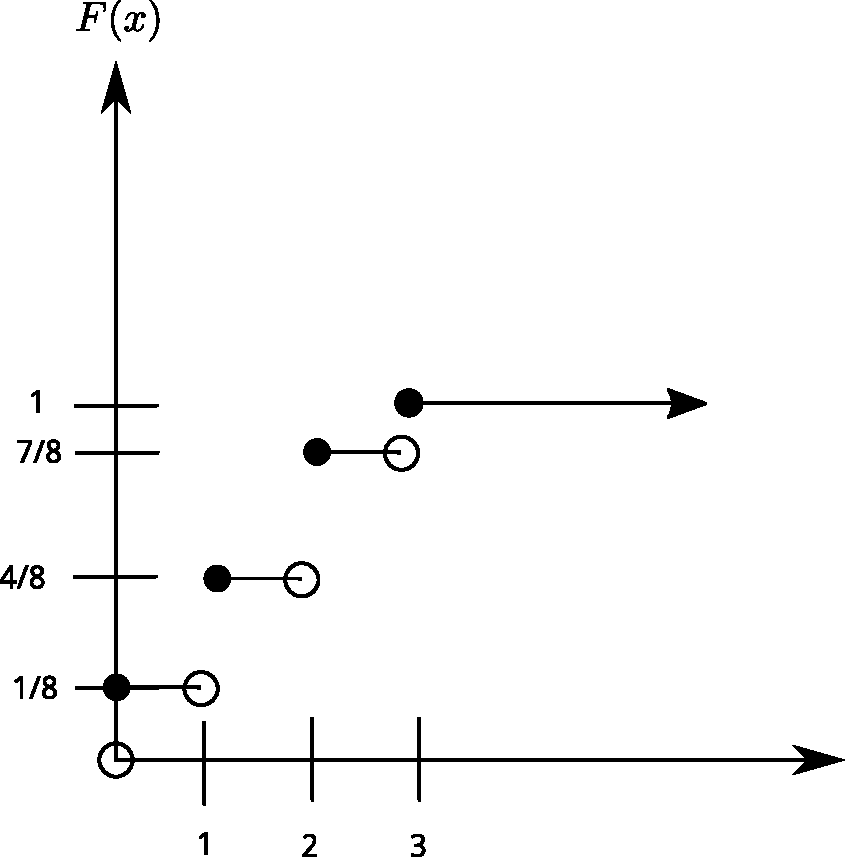
\includegraphics[width=0.4\textwidth]{./figs/cdf}
        \label{fig:s-cdf}
    \end{figure}
    \begin{align*}
	F(-0.5) = P(X \le -0.5) = 0 \\
	F(1.5) = P(X \le 1.5) = P(X \le 1) = 1/2
    \end{align*}

    \subsection*{Remark}
    \begin{itemize}
	\item $P(X \le x) = \sum\limits_{k \le x} f(k)$
	\item $F(x)$ is a nondecreasing funciton and always right continuous
	\item $0 \le F(x) \le 1$
    \end{itemize}
    
    \begin{theo}
	$\lim_{x \to -\infty} F(x) = 0$  $\lim_{x \to \infty} F(x) = 1$ \\
	Notate : pmf and CDF defines the distribution of a R.V.
	\begin{align*}
	    X &\sim f(x) \\
	    X &\sim F(x)
	\end{align*}
	where $\sim$ means "has distribution defined by"
    \end{theo}	

    Def : expected value
    \[
	E(x) = \sum\limits_{X} xf(x)
    \] 
    Ex : 
    \begin{table}[H]
        \centering
        \label{tab:expect}
        \begin{tabular}{c|cccc}
	    $x$ & 0 & 1 & 2 & 3 \\
	    \hline
	    $f(x)$ & 1/8 & 3/8 & 3/8 & 1/8
        \end{tabular}
    \end{table}
    \begin{align*}
	E(X) &= 0 \cdot 1/8 + 1 \cdot 3/8 + 2 \cdot 3/8 + 3 \cdot 1/8 \\
	&= 1.5
    \end{align*}

    The expected Value is a "weighted average" or the "center" or the distribution or a long run average

    Notate : $\mu = E(X) = \mu_X = $ mean

    Ex : Y is a R.V. w/ pmf defined 
    \begin{align*}
	f(y) = 
	\begin{cases}
	    1/N & 1, 2, \ldots, N \text{ where } N \ge 1 \text{ and } N \in \Z \\
	    0 & otherwise
	\end{cases}
    \end{align*}
    \begin{enumerate}
        \item support of $Y : 1, 2, \ldots, N$ 
	\item f(y) is a valid pmf?
    \end{enumerate}
    \begin{align*}
	0 \le f(y) \le 1 \implies 0 \le 1/N \le 1 \checkmark \\
	\sum\limits_{Y} 1/N = 1/N + 1/N + \ldots + 1/N = N(1/N) = 1 \checkmark
    \end{align*}
    Find CDF
    \begin{align*}
	F(y) &= P(Y \le y ) = \sum\limits_{k \le y} 1/N \\
	F(1) &= 1/N \\
	F(2) &= 2/N \\
	F(2.5) &= 2/N \\
	F(y) &= \lfloor y \rfloor / N \text{ where } \lfloor y \rfloor = \left\lfloor  of y when y \ge 0 \right\rfloor \\
	F(y) &= 0 \text{ when } y < 0
    \end{align*}
    \begin{figure}[H]
        \centering
        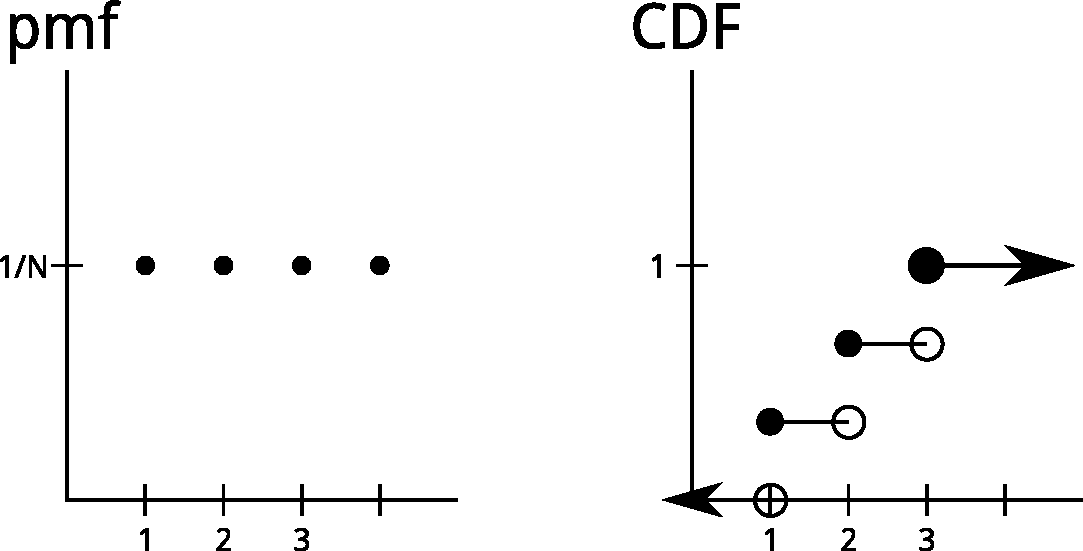
\includegraphics[width=0.8\textwidth]{./figs/floor}
        \label{fig:s-floor}
    \end{figure}
    \begin{align*}
	E(Y) &= 0f(0) + 1f(1) + \ldots + Nf(N) \\
	&= 0 \cdot 0/N + 1 \cdot 1/N + \ldots + N/N \\
	&= 1/N(1 + 2 + \ldots + N) \\
	&= 1/N(\frac{N(N + 1)}{2}) = \frac{N + 1}{2}
    \end{align*}

    \section*{Continuous R.V.}
    Recall CDF for discrete R.V. is a step function
    Def : A R.V. $X$ is called a continuous R.V. if the CDF is a continuous function There is a function $f(x)$ s.t.
    \[
	F(x) = \int_{-\infty}^{x} f(t) dt \qquad F^{\prime} (x) = f(x)
    \] 
    We don't have pmf
    \[
	P(X = x) 0 \text{ for continuous}
    \] 
    instead we have pdf (probability density function)

    Remark : for continuous R.V. 
    \begin{align*}
	P(a \le X \le b) &= P(X \le b) - P(X \le a) = F(b) - F(a) = P(a < X < b) \\
			 &= \int_{a}^{b} f(x) dx
    \end{align*}

\end{document}
